% title: The three building blocks of autoform
% description: Types and spaces define representations for values and their changes or feedback. Operations compose into programs. Transformations use spaces and operation rules to turn one program IR into another.
\documentclass[tikz,border=5pt]{standalone}
\usetikzlibrary{arrows.meta,calc,shapes.geometric}
\definecolor{numeric}{HTML}{4477AA}
\definecolor{textual}{HTML}{AA4499}

\tikzset{
    box/.style={draw, line width=0.8pt, minimum height=0.8cm,
                minimum width=1.8cm, inner sep=6pt, align=center},
    ir/.style={box},
    flow/.style={-{Stealth[length=5pt]}, line width=0.9pt},
    feedback/.style={flow, dashed},
    note/.style={font=\small, align=center},
    choice/.style={diamond, draw, line width=0.8pt,
                   aspect=2, inner sep=2pt, align=center},
}

\newcommand{\irframe}[2]{
    \draw[line width=0.8pt] #1 rectangle #2;
}

\newcommand{\transformarrow}[4][above]{
    \draw[flow] (#2) -- node[#1=6pt,note] {#4} (#3);
}


\begin{document}
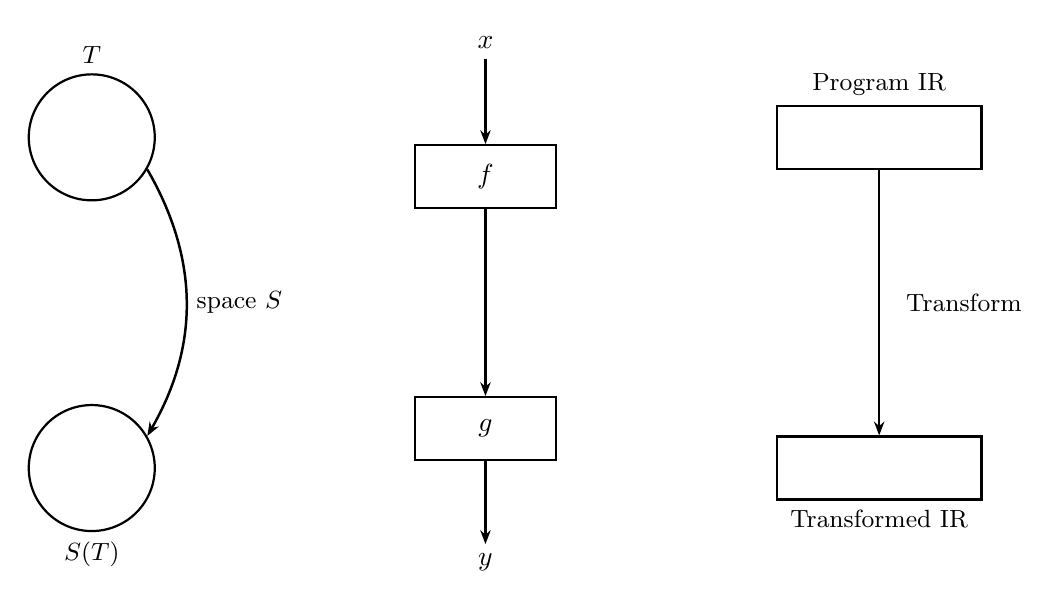
\begin{tikzpicture}
    \node[draw, circle, line width=0.8pt, minimum size=1.6cm,
          label={[note]above:$T$}] (value) at (0,0) {};
    \node[draw, circle, line width=0.8pt, minimum size=1.6cm,
          label={[note]below:$S(T)$}] (mappedtype) at (0,-4.2) {};
    \draw[flow] (value.-30) to[out=-60,in=60]
        node[right,note] {space $S$} (mappedtype.30);

    \node (x) at (5,1.2) {$x$};
    \node[box] (f) at (5,-0.5) {$f$};
    \node[box] (g) at (5,-3.7) {$g$};
    \node (y) at (5,-5.4) {$y$};
    \draw[flow] (x) -- (f);
    \draw[flow] (f) -- (g);
    \draw[flow] (g) -- (y);

    \node[ir, minimum width=2.6cm, label={[note]above:Program IR}] (original) at (10,0) {};
    \node[ir, minimum width=2.6cm, label={[note]below:Transformed IR}] (transformed) at (10,-4.2) {};
    \transformarrow[right]{original.south}{transformed.north}{Transform}
\end{tikzpicture}
\end{document}
